\section{Experimental Setup}

	The following equipment were used for the experiment:

	\begin{itemize}
	\item Constant Current Source, Model: CCS-01
	\item Low Current Source, Model LCS-02
	\item D.C. Microvoltmeter, Model DMV-001
	\item Four Probe Arrangement
	\item Thermocouple sensor
	\item Set of test samples and emery powder
	\item Suitable connectors for DMV and CCS/LCS
	\end{itemize}

	The connections were made as shown in Figure 2. The sample was placed on a non-conducting surface, and the four probes were gently rested on the sample and tightened in position. The voltage (V) and current (I) measurements were taken from the respective digital displays.

	When temperature changes were required, the sample setup was lowered into the oven chamber, and the thermocouple sensor and oven socket were connected to the PID (Proportional-Integral-Derivative) controller. After selecting the desired oven temperature (e.g., 200°C) and turning on the mains, data collection was initiated once the Present Value (PV) stabilized to the Set Value (SV) on the PID controller.

	\begin{figure}[h]
		\centering
		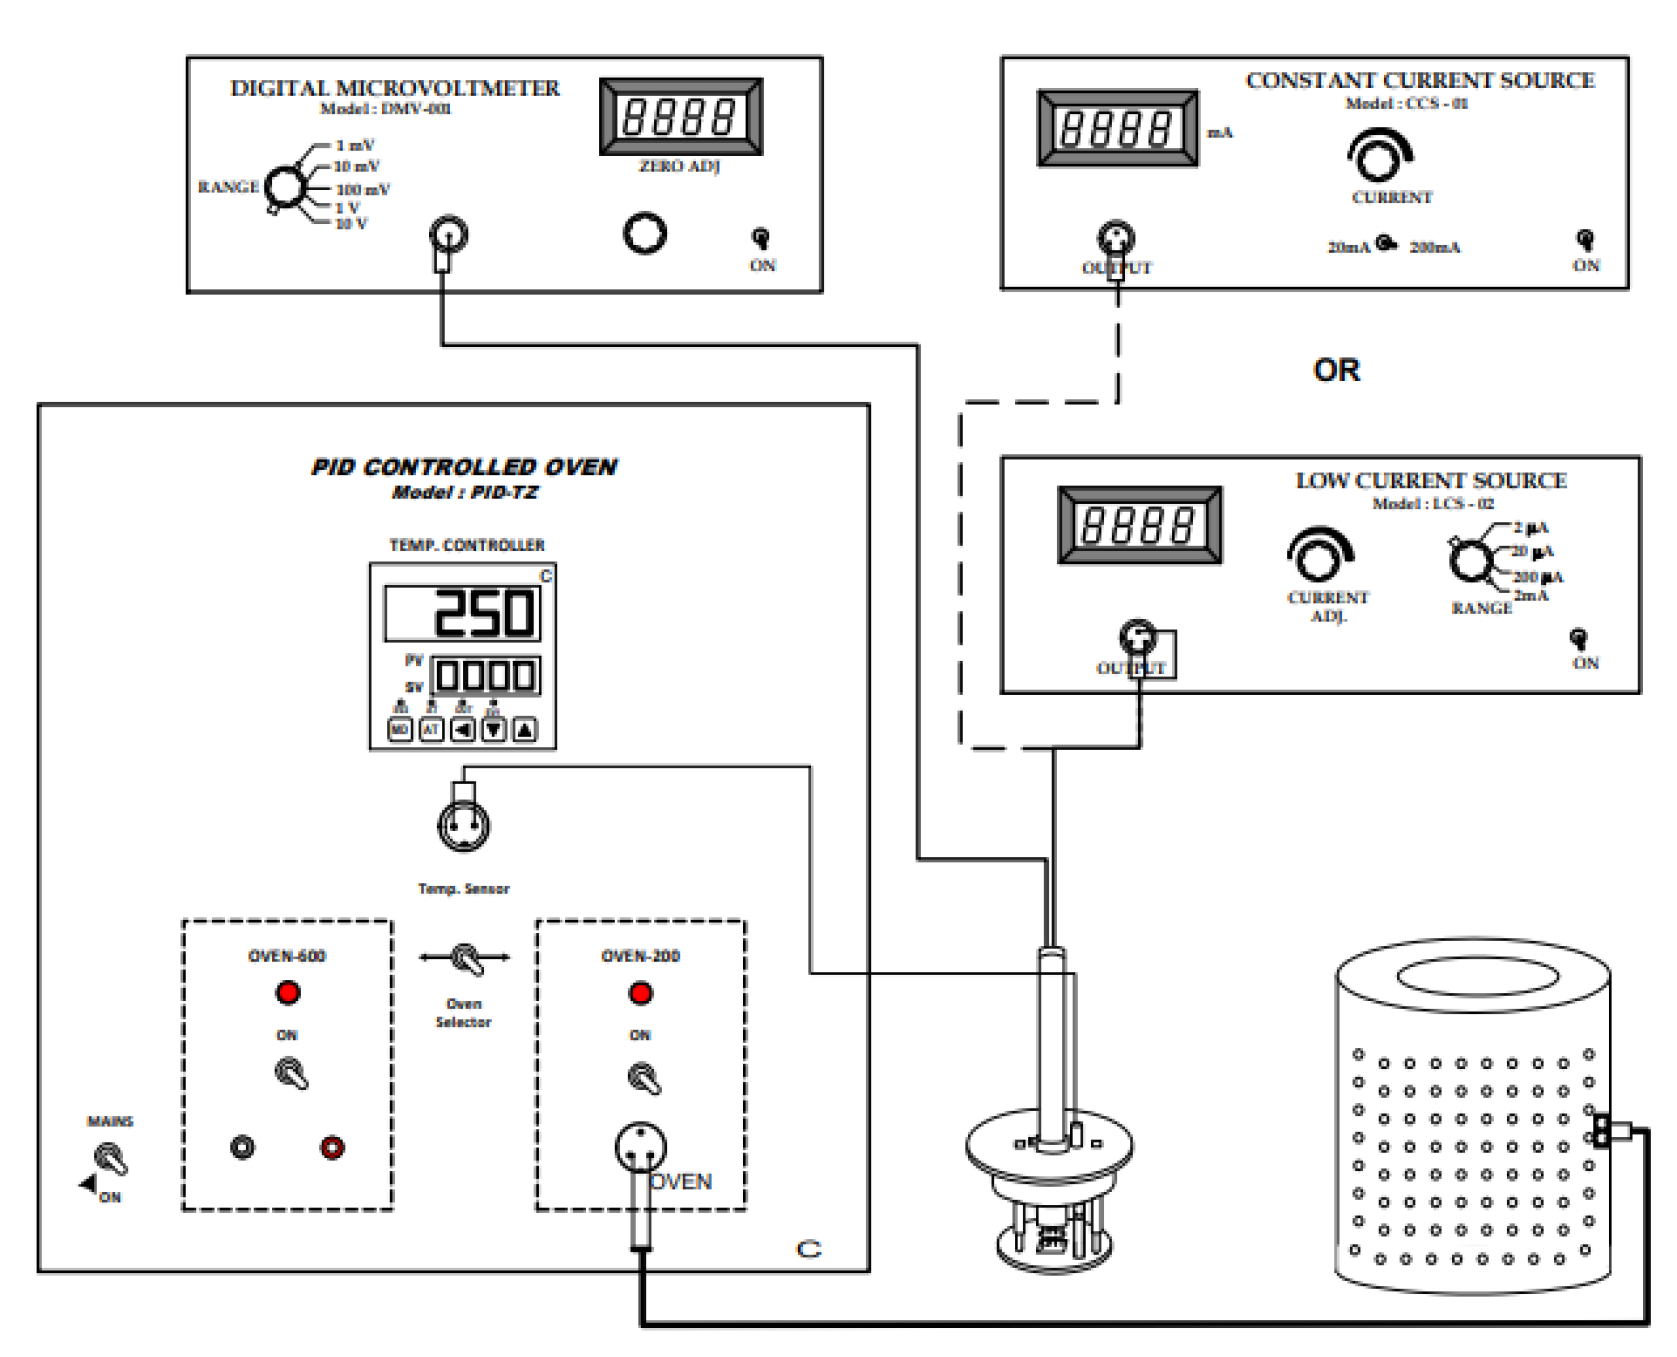
\includegraphics[width=0.8\columnwidth]{images/setup.png}
		\caption{Experimental setup for resistivity measurement with Four-Probe method.}
		\label{fig:2}
	\end{figure}